\documentclass{slide}
\usepackage{tikz}

\title{Course Overview}
\subtitle{Software Architecture}
\institute{University of Queensland}
\author{Richard Thomas}
\date{\week{1}}
\titlegraphic {
    \begin{tikzpicture}[overlay,remember picture]
    \node[left=0.1cm] at (current page.-9){
        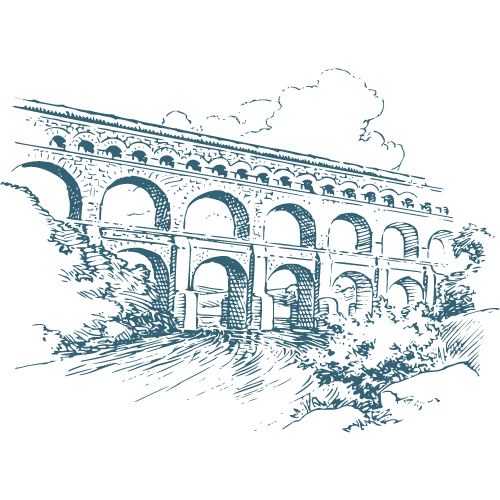
\includegraphics[width=4.75cm]{images/course-logo.png}
    };
    \end{tikzpicture}
}

\begin{document}

\maketitle

\begin{frame}{What is the course about?}
\begin{itemize}[<+->]
    \item Well, \highlight{software architecture}.
    \item Designing and building software systems, that is, multiple \highlight{software components that work together}.
    \item Using \highlight{architecture patterns} to structure software systems to be \highlight{maintainable}.
    \item How to build software that is \highlight{reliable} and \highlight{fault tolerant}.
    \item How to build software that is \highlight{scalable}.
\end{itemize}
\end{frame}


\begin{frame}{What is will we be doing?}

{\color{pine} Lectures}
\begin{itemize}[<+->]
    \item Learn common \highlight{architecture patterns}.
    \item Learn tools and techniques for \highlight{designing} and \highlight{implementing} software systems.
    \item Learn the principles for working with \highlight{distributed systems}.
\end{itemize}

{\color{pine} Tutorials}
\begin{itemize}[<+->]
    \item Work on \highlight{case studies} that implement architectual patterns.
    \item Hands-on practice with the tools and techniques for \highlight{designing} and \highlight{implementing} software systems.
\end{itemize}

{\color{pine} Practicals}
\begin{itemize}[<+->]
    \item Developing stateless and persistent \highlight{RESTful web APIs}.
    \item Packaging software components into \highlight{Docker} containers.
    \item Deploying containers to cloud platforms using \highlight{Terraform}.
    \item Using cloud platform tools to \highlight{monitor} and \highlight{scale} applications.
\end{itemize}

\end{frame}

\section{Assessment}

\begin{frame}{Assessment}

\begin{tabular}{lr}
Project Proposal & 5\% \\
Presenting an Architecture & 30\% \\
Building a Scalable Architecture & 30\% \\
Capstone Project & 35\% \\
\end{tabular}

\end{frame}

\point[Presenting an Architecture]{
    \Large
    \begin{enumerate}
        \item Find an active \highlight{open-source} project that \highlight{interests you}.
        \item \highlight{Discuss} the project with course staff.
        \item Dive into the code and \highlight{understand} the architecture.
        \item \highlight{Present} a summary of the architecture to the class.
    \end{enumerate}
}

\point[Building a Scalable Architecture]{
    \Large
    \begin{enumerate}
        \item Build a \highlight{RESTful web API} according to our API specification.
        \item \highlight{Test} that the API satisfies the specification.
        \item \highlight{Deploy} the API to a cloud platform.
        \item \highlight{Scale} the API to handle \highlight{high loads}.
    \end{enumerate}
}

\point[Capstone Project]{
    \Large
    \begin{enumerate}
        \item Write a \highlight{proposal} for a \highlight{software system} that you would like to build.
        \item Vote on other proposals that you would like to work on.
        \item Teams of 4 students will be assigned to work on a project.
        \item \highlight{Design} and \highlight{implement} the project.
    \end{enumerate}
}

\section{You and Us}

\point[Who are we?]{
    \Large
    \centering
    \begin{minipage}{0.25\textwidth}
    \begin{center}
    \begin{tikzpicture}
    \clip (0,0) circle (1.5cm) node {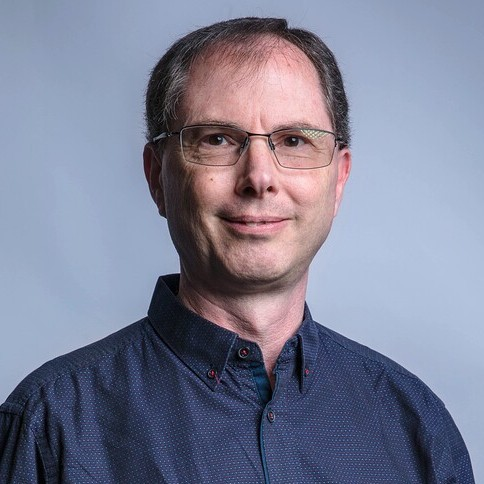
\includegraphics[width=3cm]{images/richard.jpeg}};
    \end{tikzpicture}

    Richard Thomas
    \end{center}
    \end{minipage}
%
    \begin{minipage}{0.25\textwidth}
    \begin{center}
    \begin{tikzpicture}
    \clip (0,0) circle (1.5cm) node {
\includegraphics[width=3cm]{images/brae.jpeg}};
    \end{tikzpicture}

    Brae Webb
    \end{center}
    \end{minipage}

%
    \begin{minipage}{0.25\textwidth}
    \begin{center}
    \begin{tikzpicture}
    \clip (0,0) circle (1.5cm) node {
\includegraphics[width=3cm]{images/evan.jpeg}};
    \end{tikzpicture}

    Evan Hughes
    \end{center}
    \end{minipage}
%
    \begin{minipage}{0.25\textwidth}
    \begin{center}
    \begin{tikzpicture}
    \clip (0,0) circle (1.5cm) node {
\includegraphics[width=3cm]{images/matt.png}};
    \end{tikzpicture}

    Matt Holloway
    \end{center}
    \end{minipage}
}

\question{Who are \highlight{you}?}

%\image[height=\textheight]{images/courses_with_duals.png}

%\image[height=\textheight]{images/majors.png}

%\image{images/previous_courses.png}

%\image{images/year_of_study.png}

%\image{images/important_courses.png}

\point[Course Website]{
    \Large
    All course material is hosted on the course website:
    {\color{pine}\url{https://csse6400.uqcloud.net}}

    \hfill

    If you find any \highlight{errors} or have any \highlight{improvements},
    please submit a pull request on GitHub:
    {\color{pine}\url{https://github.com/CSSE6400/software-architecture}}
}


%\references{articles,books}

\end{document}
